%!TEX root = ../../../Thesis.tex
\chapter{Colored Range Searching in Linear Space}



\begin{infosection}
    \begin{authors}
        Roberto Grossi\uni{1}\footnote{Partially supported by Italian MIUR PRIN project AMANDA.} \qquad S{\o}ren Vind\uni{2}\footnote{Supported by a grant from the Danish National Advanced Technology Foundation.}
    \end{authors}

    \begin{uninames}
        \uni{1} Universit\`{a} di Pisa \\
        \uni{2} Technical University of Denmark
    \end{uninames}

    \begin{abstract}
    In \emph{colored range searching}, we are given a set of $n$ colored points in $d \geq 2$ dimensions to store, and want to support orthogonal range queries taking colors into account. In the \emph{colored range counting} problem, a query must report the number of distinct colors found in the query range, while an answer to the \emph{colored range reporting} problem must report the distinct colors in the query range.
    
    We give the first linear space data structure for both problems in two dimensions ($d=2$) with $o(n)$ worst case query time. We also give the first data structure obtaining almost-linear space usage and $o(n)$ worst case query time for points in $d > 2$ dimensions. Finally, we present the first dynamic solution to both counting and reporting with $o(n)$ query time for $d \geq 2$ and $d \geq 3$ dimensions, respectively.
    \end{abstract}
\end{infosection}

%%%%%%%%%%%%%%%%%%%%%%%%%%%%%%%%%%%%%%%%%%%%%%%%%%%%%%%%%%%%%%%%%%
%%%%%%%%%%%%%%%%%%%%%%%%%% INTRODUCTION %%%%%%%%%%%%%%%%%%%%%%%%%%
%%%%%%%%%%%%%%%%%%%%%%%%%%%%%%%%%%%%%%%%%%%%%%%%%%%%%%%%%%%%%%%%%%
\section{Introduction}
\label{sec:crc-introduction}
%
In standard range searching a set of points must be stored to support queries for any given orthogonal $d$-dimensional query box $Q$ (see \cite{de2008orthogonal} for an overview). Two of the classic problems are standard range reporting, asking for the points in $Q$, and standard range counting, asking for the number of points in $Q$. In 1993, Janardan and Lopez \cite{janardan1993generalized} introduced one natural generalisation of standard range searching, requiring each point to have a color. This variation is known as \emph{colored range searching}\footnote{Also known in the literature as \emph{categorical} or \emph{generalized} range searching.}. 
The two most studied colored problems are \emph{colored range reporting}, where a query answer must list the distinct colors in $Q$, and \emph{colored range counting}, where the number of distinct colors in $Q$ must be reported. 

As shown in Tables~\ref{tab:count}--\ref{tab:report}, there has been a renewed interest for these problems due to their applications. For example, in database analysis and information retrieval the $d$-dimensional points represent entities and the colors are \emph{classes} (or categories) of entities. Due to the large amount of entities, statistics about their classes is the way modern data processing is performed.  A colored range query works in this scenario and reports some \emph{statistical analysis} for the classes using the range on the entities as a filtering method: ``which kinds of university degrees do European workers with age between 30 and 40 years and salary between 30,000 and 50,000 euros have?''. Here the university degrees are the colors and the filter is specified by the range of workers that are European with the given age and salary. The large amount of entities involved in such applications calls for nearly \emph{linear space} data structures, which is the focus of this paper.

\begin{table}[t]
    \centering
    \begin{tabular}{c c c c c}
       %\hline
    ~Dim.~ & Query Time               & Space Usage                          & Dyn. & ~Ref.~     \\[1mm]
        \hline\\[-3mm]
    $d=1$        & $O(\log n / \log \log n)$& $O(n)$                             & $\times$ & \cite{jaja2005space} \\[1mm]
    \hline\\[-3mm]
%%    $d=2$        & $O(n)$                   & $O(n)$ &  \\
            & $O(\log^2 n)$            & $O(n^2 \log^2 n)$                    & & \cite{gupta1995further}  \\
            & $O(\log^2 n)$            & $O(n^2 \log^2 n)$                    & & \cite{kaplan2007counting} \\
    $d=2$   & $O(X \log^7 n)$          & $O((n / X)^2 \log^6 n + n \log^4 n)$ & & \cite{kaplan2007counting} \\
            & $O\left( ( \frac{\sigma}{\log n} + \frac{n}{\log ^c n} ) (\log \log ^c n)^{2+\epsilon} \right)$ & $O(n)$ & & New \\[1mm]
    \hline\\[-3mm]
            & $O(\log^{2(d-1)} n)$     & $O(n^d \log ^{2(d-1)} n)$            & & \cite{kaplan2007counting} \\
    $d> 2$  & $O(X \log^{d-1} n)$      & $O((n / X)^{2d} + n \log^{d-1} n)$   & & \cite{kaplan2007counting} \\
            & ~$O\left(( \frac{\sigma}{\log n} + \frac{n}{\log ^c n} ) (\log  \log^{c} n)^{d-1} \log \log \log ^c n\right)$~ & $O\!\left(n (\log \log^{c} n)^{d-1} \right)$ & & New \\[1mm]
     \hline\\[-3mm]
    $d\geq 2$  & $O\left( ( \frac{\sigma}{\log n} + \frac{n}{\log ^c n} ) (\log \log ^c n)^{d} \right)$ & $O\!\left(n (\log \log^{c} n)^{d-1} \right)$ & $\times$ & New \\[1mm]
        \hline\\[-3mm]
    \end{tabular}
    \caption{Known and new solutions to \emph{colored range counting}, ordered according to decreasing space use in each dimension group. Dyn. column shows if solution is dynamic.}
 \label{tab:count}
\end{table}


Curiously, counting is considered harder than reporting among the colored range queries as it is not a decomposable problem: knowing the number of colors in two halves of $Q$ does not give the query answer. This is opposed to reporting where the query answer can be obtained by merging the list of colors in two halves of $Q$ and removing duplicates. For the standard problems, both types of queries are decomposable and solutions to counting are generally most efficient.

In the following, we denote the set of $d$-dimensional points by $P$ and let $n = |P|$. The set of distinct colors is $\Sigma$ and  $\sigma = |\Sigma| \leq n$, with $k \leq \sigma$ being the number of colors in the output. We use the notation $\log^a b = (\log b)^a$ and adopt the RAM with word size $w = \Theta(\log n)$ bits, and the size of a data structure is the number of occupied words. 

Observe that for both colored problems, the trivial solution takes linear time and space, storing the points and looking through all of them  to answer the query. Another standard solution is to store one data structure for all points of each color that supports standard range emptiness queries (``is there any point inside $Q$?''). In two dimensions, this approach can answer queries in $O(\sigma \log n)$ time and linear space using a range emptiness data structure by Nekrich \cite{nekrich2009orthogonal}.
%However, this may be worse than the trivial solution, depending on $\sigma$.
However, since $\sigma = n$ in the worst case, this does not guarantee a query time better than trivial. 
Due to the extensive history and the number of problems considered, we will present our results before reviewing existing work.
%

\begin{table}[ht]
    \centering
    \begin{tabular}{c c c c c}
    %\hline
    ~Dim.~ & Query Time               & Space Usage                          & Dyn. & ~Ref.~     \\[1mm]
    \hline\\[-3mm]
    $d=1$        & $O(1+k)$         & $O(n)$              & $\times$ & \cite{nekrich2013optimal}             \\[1mm]
    \hline\\[-3mm]
                 & $O(\log n+k)$    & $O(n \log n)$       & & \cite{shi2005optimal}                 \\
    $d=2$        & $O(\log^2 n+k\log n)$    & $O(n \log n)$       & $\times$ & \cite{gupta1995further, bozanis1995new}  \\
%    $d=2$        & $O(n)$                   & $O(n)$ & Naive \\
                & $O\left( ( \frac{\sigma}{\log n} + \frac{n}{\log ^c n} ) (\log\log^c n)^{2+\epsilon}  + k\right)$ & $O(n)$  & & New \\[1mm]
     \hline\\[-3mm]
    $d\geq 2$  & $O\left( ( \frac{\sigma}{\log n} + \frac{n}{\log ^c n} ) (\log \log ^c n)^{d} + k\right)$ & $O\!\left(n (\log \log^{c} n)^{d-1} \right)$ & $\times$ & New \\[1mm]
    \hline\\[-3mm]
    $d=3$        & $O(\log ^2 n+k)$ & $O(n \log^4 n)$     & & \cite{gupta1995further}               \\
    $d> 3$      & $O(\log n+k)$    & $O(n^{1+\epsilon})$ & & \cite{van1992new, gupta1997technique} \\ 
    $d \geq 3$        & ~~$O\left(( \frac{\sigma}{\log n} + \frac{n}{\log^c n} ) (\log\log^c n)^{d-1} \log \log \log^c n + k\right)$~~ & $O\!\left(n (\log\log^c n)^{d-1}\right)$ & & New \\[1mm]
\hline\\[-3mm]
    \end{tabular}
    \caption{Known and new solutions to \emph{colored range reporting}, ordered according to decreasing space use in each dimension group. Dyn. column shows if solution is dynamic.}
\label{tab:report}
\end{table}


\subsection{Our results}
\label{sub:our-results}
%
We observe (see Section~\ref{sub:previous-results}) that there are no known solutions to any of the colored problems in two dimensions that uses $O(n)$ words of space and answer queries in $o(n)$ worst case time. Furthermore, for colored range reporting there are no known solutions in $d> 3$ dimensions using $o(n^{1+\epsilon})$ words of space and answering queries in $o(n)$ worst case time. For colored range counting, no solutions with $o(n \polylog n)$ words of space and $o(n)$ worst case time exist. 

We present the first data structures for colored range searching achieving these bounds, improving almost logarithmically over previously known solutions in the worst case (see Section~\ref{sub:previous-results} and Tables~\ref{tab:count}--\ref{tab:report}). Specifically, we obtain
\begin{itemize}
    \item $o(n)$ query time and $O(n)$ space in two dimensions,
    \item $o(n)$ query time and $o(n \polylog n)$ space for counting in $d \geq 2$ dimensions,
    \item $o(n)$ query time and $o(n^{1+\epsilon})$ space for reporting in $d > 3$ dimensions,
    \item $o(n)$ query time supporting $O(\mathrm{polylg \,} n)$ updates in $d \geq 2$ and $d \geq 3$ dimensions for counting and reporting, respectively.
\end{itemize}

%The results improve almost logarithmically over the query time of previously known solutions in linear space in the worst case. 

We note that while our bounds have an exponential dimensionality dependency (as most previous results), it only applies to $\log \log n$ factors in the bounds.
Our solutions can be easily implemented and parallelized, so they are well-suited for the distributed processing of large scale data sets. Our main results can be summarised in the following theorems, noting that $c > 1$ is an arbitrarily chosen integer, and $\sigma \leq n$ is the number of distinct colors.

%%% Two dimensions:
\begin{theorem}\label{thm:2D}
    There is a linear space data structure for two-dimensional colored range counting and reporting storing $n$ points, each assigned one of $\sigma$ colors. The data structure answers queries in time $O( ( \sigma / \log n + n / \log ^c n ) (\log \log ^c n)^{2+\epsilon} )$, with reporting requiring an additive term $O(k)$.
\end{theorem}

%%% Many dimensions:
\begin{theorem}\label{thm:dD}
  There is a $O(n (\log \log ^{c} n) ^{d-1})$ space data structure storing $n$ $d$-dimensional colored points each assigned one of $\sigma$ colors. Each colored range counting and reporting query takes time $O(( \sigma / \log n + n / \log ^c n ) (\log \log ^{c} n) ^{d-1} \log \log \log ^c n )$. Reporting requires an additive $O(k)$ time.
\end{theorem}

To obtain these results, we partition points into groups depending on their color. Each group stores all the points for at most $\log n$ specific colors. Because the colors are partitioned across the groups, we can obtain the final result to a query by merging query results for each group (and we have thus obtained a decomposition of the problem along the color dimension). A similar approach was previously used in \cite{kaplan2007counting}.

In order to reduce the space usage of our data structure, we partition the points in each group into a number of buckets of at most $\log^c n$ points each. The number of buckets is $O(\sigma / \log n + n / \log ^c n)$, with the first term counting all underfull buckets and the second counting all full buckets. Each bucket stores $m \leq \log ^c n$ points colored with $f \leq \log n$ different colors.
%Our approach partitions points into groups depending on their color. Each group stores all points of $\leq \log n$ specific colors. A further subdivision of the groups into buckets ensures that the number of points in each bucket is $O(\log ^c n)$. Thus, the number of buckets is $O(\sigma / \log n + n / \log ^c n)$ (the first term counts all underfull buckets, the second counts all full buckets). Because the colors are partitioned across the groups, we can obtain the final result to a query by summing the number of colors found in each group (and we have thus obtained a decomposition of the problem along the color dimension). 
%As the colors of each group may be present in several buckets, we cannot obtain the solution for a group from an individual count for each bucket (since we risk counting a color several times). 
%Instead, we use an efficient solution to the $d$-dimensional \emph{colored range reporting problem} in the buckets (where the number of points is $m \leq \log ^c n$ and the number of colors is $f \leq \log n$). 
To avoid counting a color several times across different buckets, we use a solution to the $d$-dimensional colored range reporting problem in each bucket for which answers to queries are given as bitstrings. Answers to the queries in buckets can be merged efficiently using bitwise operations on words.
%and require that the answer to a query is given as a $f$-bit long bitstring. Since $f \leq w$, we can use bitwise OR operations to efficiently compose the answers to each of the queries on the buckets to produce the full answer for the group. 
We finally use an $o(n)$ space lookup table to obtain the count or list of colors present in the merged answer. 
%This takes constant time per answer found in the lookup table.

The solution to $d$-dimensional colored range reporting for each bucket is obtained by building a $d$-dimensional range tree for the $m$ points, which uses a new linear space and $O(\log \log m)$ time solution to restricted one-dimensional colored range reporting as the last auxiliary data structure. In total, each bucket requires $O(m \log ^{d-1} m)$ space and $O(\log ^{d-1} m \log \log m)$ query time. In two dimensions, we reduce the space to linear by only storing representative rectangles in the range tree covering $O(\log m)$ points each. Using the linear space range reporting data structure by Nekrich \cite{nekrich2009orthogonal}, we enumerate and check the underlying points for each of the $O(\log m)$ range tree leaves intersecting the query range, costing us a small penalty of $O(\log ^{\epsilon} n)$ per point. We thus obtain a query time of $O(\log ^{2+\epsilon} m)$ for two-dimensional buckets in linear space.

% Though the basic approach is simple, it allows us to give in Theorem % \ref{thm:2D} the first linear space data structure with $o(n)$ worst % case query time for two-dimensional colored range counting and colored % range reporting. Furthermore, Theorem \ref{thm:dD} is the first % almost-linear space data structure for both colored range counting and % colored range reporting in higher dimensions with $o(n)$ worst case % query time. 
% \fxfatal{Comparison needs to be improved.}

\vspace{0.5em}
Using classic results on dynamisation of range trees, we can dynamise the data structure with a little additional cost in query time. Previously, there was no known dynamic data structures with $o(n)$ query time for colored range counting in $d \geq 2$ dimensions and colored range reporting in $d \geq 3$ dimensions. Consequently, this is the first such dynamic data structure.

%%% Dynamic:
\begin{theorem}\label{thm:dyn-dD}
    There is a dynamic $O(n (\log \log ^{c} n) ^{d-1})$ space data structure storing $n$ $d$-dimensional colored points each assigned one of $\sigma$ colors. The data structure answers colored range counting and reporting queries in time $O(( \sigma / \log n + n / \log ^c n ) (\log \log ^{c} n) ^{d})$. Reporting requires a additive $O(k)$ time and updates are supported in $O((\log \log ^c n) ^d)$ amortised time.
\end{theorem}

Finally, if paying a little extra space, we can get a solution to the problem where the query time is bounded by the number of distinct colors instead of the number of points. This is simply done by not splitting color groups into buckets, giving the following result. 

%%% Colors
\begin{corollary}\label{thm:col-dD}
    There is a $O(n \log ^{d-1} n)$ space data structure for $n$ $d$-dimensional colored points each assigned one of $\sigma$ colors. The data structure answers colored range counting and reporting queries in time $O(\sigma \log ^{d-2} n \log \log n)$. Reporting requires a additive $O(k)$ time.
\end{corollary}

In two dimensions this is a logarithmic improvement over the solution where a range emptiness data structure is stored for each color at the expense of a $\log n$ factor additional space. The above approach can be combined with the range emptiness data structure by Nekrich \cite{nekrich2009orthogonal} to obtain an output-sensitive result where a penalty is paid per color reported:

%%% Colors, output-sensitive
\begin{corollary}\label{thm:col-2D}
    There is a $O(n \log n)$ space data structure storing $n$ two-dimensional colored points each assigned one of $\sigma$ colors. The data structure answers colored range counting and reporting queries in time $O(\sigma + k \log n \log \log n)$.
\end{corollary}

\subsection{Previous results}
\label{sub:previous-results}
\paragraph*{Colored range counting.}
%
Colored range counting is challenging, with a large gap in the known bounds compared to standard range counting, especially in two or more dimensions. For example, a classic range tree solves two-dimensional standard range counting in logarithmic time and $O(n \log n)$ space, but no polylogarithmic time solutions in $o(n^2)$ space are known for colored range counting.

Larsen and van Walderveen \cite{larsen2013near, gupta1995further} showed that colored range counting in one dimension is equivalent to two-dimensional standard range counting. Thus, the optimal $O(\log n / \log \log n)$ upper bound for two-dimensional standard range counting by J{\'a}J{\'a} et al. \cite{jaja2005space} which matches a lower bound by Patrascu \cite{patrascu2007lower} is also optimal for one-dimensional colored range counting.

In two dimensions, Gupta et al. \cite{gupta1995further} show a solution using $O(n^2 \log^2 n)$ space that answers queries in $O(\log^2 n)$ time. They obtain their result by storing $n$ copies of a data structure which is capable of answering three-sided queries. The same bound was matched by Kaplan et al. \cite{kaplan2007counting} with a completely different approach in which they reduce the problem to standard orthogonal range counting in higher dimensions. Kaplan et al. also present a tradeoff solution with $O(X \log^7 n)$ query time and $O((\frac{n}{X})^2 \log^6 n + n \log^4 n)$ space for $1 \leq X \leq n$. Observe that the minimal space use for the tradeoff solution is $O(n \log^4 n)$.

In $d > 2$ dimensions, the only known non-trivial solutions are by Kaplan et al. \cite{kaplan2007counting}. One of their solutions answers queries in $O(\log ^{2(d-1)} n)$ time and $O(n^d \log ^{2(d-1)} n)$ space, and they also show a number of tradeoffs, the best one having $O(X \log^{d-1} n)$ query time and using $O((\frac{n}{X})^{2d} + n \log^{d-1} n)$ space for $1 \leq X \leq n$. In this case, the minimal space required by the tradeoff is $O(n \log ^{d-1} n)$.

Kaplan et al. \cite{kaplan2007counting} showed that answering $n$ two dimensional colored range counting queries in $O(n^{p/2})$ time (including all preprocessing time) yields an $O(n^p)$ time algorithm for multiplying two $n \times n$ matrices. For $p < 2.373$, this would improve the best known upper bound for matrix multiplication \cite{williams2012multiplying}. Thus, solving two dimensional colored range counting in polylogarithmic time per query and $O(n \polylog n)$ space would be a major breakthrough. This suggest that even in two dimensions, no polylogarithmic time solution may exist.

%Finally, Lai et al. presented a randomised approximate solution to colored range counting in $d$ dimensions, answering queries in time $O(d \log^{d+1} n)$ and space $O(dn \log ^{d-1} n)$ \cite{lai2005approximate,lai2008approximate}. Their data structure is randomized in the sense that the answer is expected to be correct to within a constant factor of the correct answer. 
%\fxfatal{SV: Removed approximate thing, as it does not really fit into anything. Check if you agree.}
% RG: removed  $\epsilon$  as we use for another purpose


\paragraph*{Colored range reporting.}
%
The colored range reporting problem is relatively well-studied \cite{janardan1993generalized, nekrich2012space, nekrich2013optimal, nekrich2014efficient, gagie2012colored, shi2005optimal, gupta1995further, gupta1997technique, van1992new, mortensen2003generalized, bozanis1995new, larsen2012efficient}, with output-sensitive solutions almost matching the time and space bounds obtained for standard range reporting in one and two dimensions. In particular, Nekrich and Vitter recently gave a dynamic solution to one dimensional colored range reporting with optimal query time $O(1+k)$ and linear space \cite{nekrich2013optimal}, while Gagie et al. earlier presented a succinct solution with query time logarithmic in the length of the query interval \cite{gagie2012colored}.

In two dimensions, Shi and JaJa obtain a bound of $O(\log n + k)$ time and $O(n \log n)$ space \cite{shi2005optimal} by querying an efficient static data structure for three-sided queries, storing each point $O(\log n)$ times. Solutions for the dynamic two-dimensional case were developed in \cite{gupta1995further, bozanis1995new}, answering queries with a logarithmic penalty per answer. If the points are located on an $N \times N$ grid, Agarwal et al. \cite{agarwal2002range} present a solution with query time $O(\log \log N + k)$ and space use $O(n \log ^2 N)$. Gupta et al. achieve a static data structure using $O(n \log ^4 n)$ space and answering queries in $O(\log ^2 n + k)$ \cite{gupta1995further} in the three-dimensional case. To the best of our knowledge, the only known non-trivial data structures for $d> 3$ dimensions are by van Kreveld and Gupta et al., answering queries in $O(\log n + k)$ time and using $O(n^{1+\epsilon})$ space \cite{van1992new, gupta1997technique}. Other recent work on the problem include external memory model solutions when the points lie on a grid \cite{nekrich2012space, larsen2012efficient, nekrich2014efficient}.

% The paper is structured with Section \ref{sec:basics} giving the basic % approach using grouping and bucketing and reducing the problem to % restricted colored range reporting, proving Theorem \ref{thm:dD}. % Section \ref{sec:linear} proves Theorem \ref{thm:2D}, showing how to % reduce the space to linear in two dimensions. Section % \ref{sec:dynamic} shows how to dynamise the data structure and gives % Theorem \ref{thm:dyn-dD}, and Section \ref{sec:colors} show how to % obtain the color and output-sensitive bounds of Corollaries % \ref{thm:col-dD} and \ref{thm:col-2D}.


\section{Colored Range Searching in Almost-Linear Space}
\label{sec:basics}
%
We present here the basic approach that is modified to obtain our theorems. We first show how to partition the points into $O(\sigma / \log n + n / \log ^c n)$ buckets each storing $m = O(\log ^c n)$ points of $f = O(\log n)$ distinct colors, for which the results can be easily combined. We then show how to answer queries in each bucket in time $O(\log ^{d-1} m \log \log m)$ and space $O(m \log ^{d-1} m)$, thus obtaining Theorem \ref{thm:dD}.

\subsection{Color grouping and bucketing}
%
We partition the points of $P$ into a number of groups $P_i$, where $i = 1, \ldots, \frac{\sigma}{\log n}$, depending on their color. Each group stores all points having $f = \log n$ distinct colors (except for the last group which may store points with less distinct colors). For each group $P_i$ we store an ordered color list $L_i$ of the $f$ colors in the group. That is, a group may contain $O(n)$ points but the points have at most $f$ distinct colors. Since colors are partitioned among groups, we can clearly answer a colored query by summing or merging the results to the same query in each group. 
%Observe that assuming a colored range counting query can be answered for each group, we can clearly answer a colored range counting query by adding the results for each group (since colors are partitioned among groups).

\begin{figure}[tb]
	\begin{center}
	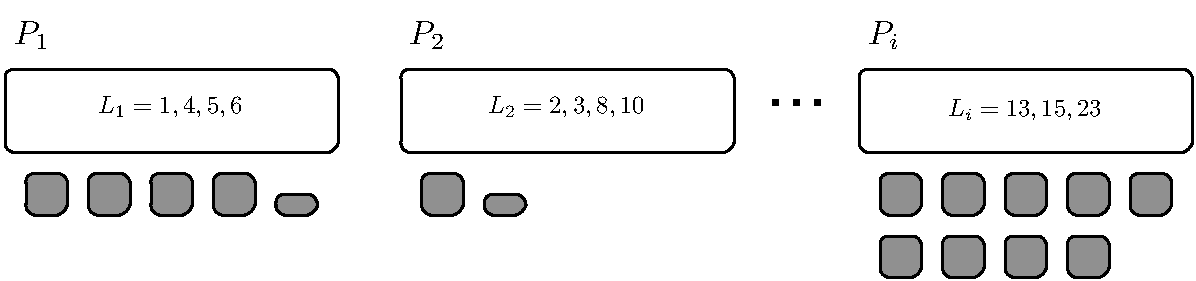
\includegraphics[width=0.9\textwidth]{chapters/papers/coloredrangecounting/groups-buckets}
	\caption{Grouping and bucketing of some point set with $f = 4$. The white boxes are the groups and the grey boxes below each group are buckets each storing $O(\log^c n)$ points.\label{fig:groups-buckets}}
	\end{center}
\end{figure} 

Each group is further partitioned into a number of buckets containing $m = \log ^c n$ points each (except for the last bucket, which may contain fewer points). Since the buckets partition the points and there cannot be more than one bucket with fewer than $\log ^c n$ points in each group, the total number of buckets is $O(\sigma / \log n + n / \log ^c n)$. See Figure \ref{fig:groups-buckets} for an example of the grouping and bucketing. 

We require that each bucket in a group $P_i$ supports answering \emph{restricted colored range reporting queries} with an $f$-bit long bitstring, where the $j$th bit indicates if color $L_i[j]$ is present in the query area $Q$ in that bucket. Clearly, we can obtain the whole answer for $Q$ and $P_i$ by using bitwise OR operations to merge answers to the restricted colored range reporting query $Q$ for all buckets in $P_i$. We call the resulting bitstring $F_{i, Q}$, which indicates the colors present in the query range $Q$ across the entire group $P_i$.
%Clearly, a constant number of bitwise OR operations per bucket is enough to produce a $f$-bit long bitstring from a single restricted colored range reporting query per bucket. We call this bitstring $F_{i, Q}$, and note that it indicates the colors present in the query range across the entire group $P_i$.

Finally, we store a lookup table $T$ of size $O(\sqrt{n} \log n) = o(n)$ for all possible bitstrings of length $\frac{f}{2}$. For each bitstring, the table stores the number of {\bitone}s present in the bitstring and the indices where the {\bitone}s are present. Using two table lookups in $T$ with the two halves of $F_{i, Q}$, we can obtain both the number of colors present in $P_i$ for $Q$, and their indices into $L_i$ in $O(1)$ time per index. 

Summarising, we can merge answers to the restricted colored range reporting queries in $O(1)$ time per bucket and obtain the full query results for each group $P_i$. Using a constant number of table lookups per group, we can count the number of colors present in $Q$. There is $O(1)$ additional cost per reported color.
%Summarising, we can combine answers from each bucket in a group and add the results for all groups in time linear in the number of buckets for a colored range counting query. Thus, the total time spent is bounded by the number of buckets present multiplied by the time taken to answer a restricted colored range reporting query in a bucket. Additionally, we can answer colored range reporting queries in the same time plus $O(1)$ time per reported color.

\subsection{Restricted colored range reporting for buckets}
\label{sec:RCRR}
%
Each bucket in a group $P_i$ stores up to $m = \log^c n$ points colored with up to $f = \log n$ distinct colors, and must support restricted colored range reporting queries, reporting the colors in  query range $Q$ using an $f$-bit long bitstring. A simple solution is to use a classic $d$-dimensional range tree $R$, augmented with an $f$-bit long bitstring for each node on the last level of $R$ (using the $L_i$ ordering of the $f$ colors). The colors within the range can thus be reported by taking the bitwise OR of all the bitstrings stored at the $O(\log^d m)$ summary nodes of $R$ spanning the range in the last level. This solution takes total time $O(\frac{f}{w} \log ^d m) = O(\log ^d m)$ and space $O(m \log ^{d-1} m \frac{f}{w}) = O(m \log ^{d-1} m)$, and it can be constructed in time $O(m \log ^{d-1} m)$ by building the node bitstrings from the leaves and up (recall that $w = \Theta(\log n)$ is the word size). 

The above solution is enough to obtain some of our results, but we can improve it by replacing the last level in $R$ with a new data structure for restricted one-dimensional colored range reporting over integers that answer queries in time $O(\log \log m)$ and linear space. A query may perform $O(\log ^{d-1} m)$ one-dimensional queries on the last level of the range tree, so the query time is reduced to $O(\log ^{d-1} m \log \log m)$ per bucket. The new data structure used at the last level is given in the next section.

Observe that though the points are not from a bounded universe, we can remap a query in a bucket to a bounded universe of size $m$ in time $O(\log m)$ and linear space per dimension. We do so for the final dimension, noting that we only need to do it once for all $O(\log ^{d-1} m)$ queries in the final dimension. 

\subsubsection*{1D restricted colored range reporting on integers.}
%
Given $O(m)$ points in one dimension from a universe of size $m$, each colored with one of $f = \log n$ distinct colors, we now show how to report the colors contained in a query range in $O(\log \log m)$ time and linear space, encoded as an $f$-bit long bitstring. First, partition the points into $j = O(m / \log m)$ intervals spanning $\Theta(\log m)$ consecutive points each. Each interval is stored as a balanced binary search tree of height $O(\log \log m)$, with each node storing a $f$-bit long bitstring indicating the colors that are present in its subtree. Clearly, storing all these trees take linear space.

We call the first point stored in each interval a \emph{representative} and store a predecessor data structure containing all of the $O(m / \log m)$ representatives of the intervals. Also, each representative stores $O(\log m)$ $f$-bit long bitstrings, which are summaries of the colors kept in the $1, 2, \ldots, 2^{\log j}$ neighboring intervals. We store these bitstrings both towards the left and the right from the representative, in total linear space.


A query $[a, b]$ is answered as follows. 
We decompose the query into two parts, first finding the answer for all intervals fully contained in $[a, b]$, and then finding the answer for the two intervals that only intersect $[a, b]$. 
%We find two bitstrings summarising the answer for all intervals fully contained in $[a, b]$ and merge the result with bitstrings for the two intervals that intersect but are not fully contained in $[a, b]$. 
The first part is done by finding the two outermost representatives inside the interval (called $a', b'$, where $a \leq a' \leq b' \leq b$) by using predecessor queries with $a$ and $b$ on the representatives. 
%We first at most two bitstrings that are stored at the representatives and that cover the largest portion of $[a, b]$. This is equivalent to finding the two outermost intervals that are fully covered by $[a,b]$, which is done using predecessor/successor queries with $a$ and $b$ on the representatives. 
Since we store summaries for all power-of-2 neighboring intervals of the representatives, there are two bitstrings stored with $a'$ and $b'$ which summarises the colors in all fully contained intervals. 

To find the answer for the two intervals that contain $a$ or $b$, we find $O(\log \log m)$ nodes of the balanced binary tree for the interval and take the bitwise OR of the bitstrings stored at those nodes in $O(\log \log m)$ total time. Using one of the classic predecessor data structures \cite{van1976design, mehlhorn1990bounded, willard1983log} for the representatives, we thus obtain a query time of $O(\log \log m)$ and linear space.
%The colors found in the two intervals that contain $a$ and $b$ to obtain the final answer. That is, we find the bitstring answer for the two intervals $[a, a']$ and $[b', b]$ and merge these with the bitstring answers for interval $[a', b']$. The bitstring for $[a, a']$ or $[b', b]$ is determined by


\section{2D Colored Range Searching in Linear Space}
\label{sec:linear}
%
To obtain linear space in two dimensions and the proof of Theorem~\ref{thm:2D}, we use the same grouping and bucketing approach as in Section~\ref{sec:basics}. For each group $P_{i'}$, we only change the solution of each bucket $B_i$ in $P_{i'}$, recalling that $B_i$ contains up to $m = \log^c n$ points with $f = \log n$ distinct colors, so as to use linear space instead of $O(m \log m)$ words of space. 

We store a linear space 2D standard range reporting data structure $A_i$ by Nekrich~\cite{nekrich2009orthogonal} for all points in the bucket $B_i$. As shown in~\cite{nekrich2009orthogonal}, $A_i$ supports orthogonal standard range reporting queries in $O(\log m + r \log ^{\epsilon} m)$ time and updates in $O(\log ^{3+\epsilon} m)$ time, where $r$ is the reported number of points and $\epsilon > 0$.


% \begin{theorem}[Nekrich % \cite{nekrich2009orthogonal}]\label{thm:nekrich}
%     There is a linear space data structure storing $n$ two-dimensional % points which support orthogonal standard range reporting queries in % $O(\log n + k \log ^{\epsilon} n)$ time and updates in $O(\log % ^{3+\epsilon} n)$ time, where $k$ is the reported number of points and % $\epsilon > 0$.
% \end{theorem}

We also store a simple 2D range tree $R_i$ augmented with $f$-bit long bitstrings on the last level as previously described in Section~\ref{sec:RCRR}, but instead of storing points in $R_i$, we reduce its space usage by only storing areas covering $O(\log m)$ points of $B_i$ each. This can be done by first building $R_i$ taking $O(m \log m)$ space and time, and then cutting off subtrees at nodes at maximal height (called cutpoint nodes) such that at most $c' \log m$ points are covered by each cutpoint node, for a given constant $c'>0$. In this way, each cutpoint node is implicitly associated with $O(\log m)$ points, which can be succinctly represented with $O(1)$ words as they all belong to a distinct 2D range. Note that the parent of a cutpoint node has $\Omega(\log m)$ descending points, hence there are $O(m/\log m)$ cutpoint nodes.

A query is answered by finding $O(\log^2 m)$ summary nodes in $R_i$ that span the entire query range $Q$. Combining bitstrings as described in Section~\ref{sec:RCRR}, the colors for all fully contained ranges that are not stored in the leaves can thus be found. Consider now one such leaf $\ell$ covering an area intersecting $Q$: since the $O(\log m)$ points spanned by $\ell$ may not be all contained in $Q$, we must check those points individually. Recall that the points associated with $\ell$ are those spanning a certain range $Q'$, so they can be succinctly represented by $Q'$. To actually retrieve them, we issue a query $Q'$ to $A_i$, check which ones belong to $Q' \cap Q$, and build a bitstring for the colors in $Q' \cap Q$. We finally merge the bitstrings for all summary nodes and intersecting leaves in constant time per bitstring to obtain the final result.

The time spent answering a query is $O(\log ^2 m)$ to find all bitstrings in non-leaf nodes of $R_i$ and to combine all the bitstrings. The time spent finding the bitstring in leaves is $O(\log ^{1+\epsilon} m)$ per intersecting leaf as we use Nekrich's data structure $A_i$ with $r = O(\log m)$. Observe that only two leaves spanning a range of $O(\log m)$ points may be visited in each of the $O(\log m)$ second level data structures visited, so the time spent in all leaves is $O(\log ^{2+\epsilon} m)$, which is also the total time. Finally, since we reduced the size of the range tree by a factor $\Theta(\log m)$, the total space usage is linear. This concludes the proof of Theorem \ref{thm:2D}. 
%For higher dimension, we will show in the full version of the paper how to extend our approach using the data structure of Karpinski, Nekrich 2009.
%\fxfatal{Fix the reference}
% NOTE: I have not found any non-grid based $d>2$ and almost-linear space range reporting data structures. Thus left out.


% \begin{itemize}
%     \item Same approach can be used for higher dimensions (Karpinski, % Nekrich 2009): Not to linear space, but reducing space usage to $O(m % \log ^{d-2+\epsilon} m)$ per bucket.
%     \item In particular, in three dimensions, we can obtain a solution % with X space use and Y query time. \fxfatal{Probably not an % interesting note.}
% \end{itemize}

\section{Dynamic Data Structures}
\label{sec:dynamic}
%
We now prove Theorem~\ref{thm:dyn-dD} by discussing how to support operations $\opins(p, c)$ and $\opdel(p)$, inserting and deleting a point $p$ with color $c$, respectively. Note that the color $c$ may be previously unused. We still use parameters $f$ and $m$ to denote the number of colors in groups and points in buckets, respectively.
We first give bounds on how to update a bucket, and then show how to support updates in the color grouping and point bucketing. 

% We also give bounds when the buckets are implemented with the classic % range tree where each node on the final level is augmented with an % $f$-bit long bitstring over the colors in the subtree. 

\subsection{Updating a bucket}
%
Updating a bucket with a point corresponds to updating a $d$-dimensional range tree using known techniques in dynamic data structures. Partial rebuilding \cite{andersson1999general, overmars1983design} requires amortised time $O(\log^d m)$, including updating the bitstrings in the partially rebuilt trees and in each node of the last level trees (which takes constant time). Specifically, the bitstrings for the $O(\log^{d-1} m)$ trees on the last level where a point was updated may need to have the bitstrings fixed on the path to the root on that level. This takes time $O(\log m)$ per tree, giving a total amortised update time of $O(\log^d m)$.

\subsection{Updating color grouping and point bucketing}
\label{sub:update-color-group-bucket}
%
When supporting $\opins(p, c)$, we first need to find the group to which $c$ belongs. If the color is new and there is a group $P_i$ with less than $f$ colors, we must update the color list $L_i$. Otherwise, we can create a new group $P_i$ for the new color. In the group $P_i$, we must find a bucket to put $p$ in. If possible, we put $p$ in a bucket with less than $m$ points, or otherwise we create a new bucket for $p$. Keeping track of sizes of groups and buckets can be done using priority queues in time $O(\log \log n)$. Note that we never split groups or buckets on insertions.

As for supporting $\opdel(p)$, we risk making both groups and buckets underfull, thus requiring a merge of either. A bucket is underfull when it contains less than $m/2$ points. We allow at most one underfull bucket in a group. If there are two underfull buckets in a group, we merge them in time $O(m \log^d m)$. Since merging buckets can only happen after $\Omega(m)$ deletions, the amortized time for a deletion in this case is $O(\log^d m)$. A group is underfull if it contains less than $f/2$ colors and, as for buckets, if there are any two underfull groups $P_i, P_j$, we merge them. When merging $P_i, P_j$ into a new group $P_r$, we concatenate their color lists $L_i, L_j$ into $L_r$, removing the colors that are no more present while keeping the relative ordering of the surviving colors from $L_i, L_j$. In this way, a group merge does not require us to merge the underlying buckets, as points are partitioned arbitrarily into the buckets. However, a drawback arises: as the color list $L_r$ for the merged group is different from the color lists $L_i, L_j$ used for answering bucket queries, this may introduce errors in bucket query answers. Recall that an answer to a bucket query is an $f$-bit long bitstring which marks with {\bitone}s the colors in $L_i$ that are in the range $Q$. So we have a bitstring for $L_i$, and one for $L_j$, for the buckets previously belonging to $P_i, P_j$, but we should instead output a bitstring for $L_r$ in time proportional to the number of buckets in $P_r$. We handle this situation efficiently as discussed in Section~\ref{sub:fixing-bucket-answers}.

\subsection{Fixing bucket answers during a query}
\label{sub:fixing-bucket-answers}
%
As mentioned in Section~\ref{sub:update-color-group-bucket}, we do not change the buckets when two or more groups are merged into $P_r$. Consider the $f$-bit long bitstring $b_i$ that is the answer for one merged group, say $P'_i$, relative to its color list, say $L_i$. However, after the merge, only a sublist $L'_i \subseteq L_i$ of colors survives as a portion of the color list $L_r$ for $P_r$. We show how to use $L_i$ and $L'_i$ to contribute to the $f$-bit long bitstring $a$ that is the answer to query $Q$ for the color list $L_r$ in $P_r$. The time constraint is that we can spend time proportional to the number, say $g$, of buckets in $P_r$. 


% Observe that when merging two groups, at least $f/2$ of the bits in % any answer to a restricted colored range reporting in the buckets % belonging to the groups must be \bitzero. 


We need some additional information. For each merged group $P'_i$, we create an $f$-bit long bitstring $v_i$ with bit $j$ set to \bitone\ if and only if color $L_i[j]$ survives in $L_r$ (i.e. some point in $P_r$ has color $L_i[j]$). We call $v_i$ the \emph{possible answer bitstring} and let $o_i$ be the number of {\bitone}s in $v_i$: in other words, $L'_i$ is the sublist built from $L_i$ by choosing the colors $L_i[j]$ such that $v_i[j] = \bitone$, and $o_i = |L'_i|$. 

Consider now the current group $P_r$ that is the outcome of $h \leq f$ old merged groups, say $P'_1, P'_2, \ldots, P'_h$ in the order of the concatenation of their color lists, namely, $L_r = L'_1 \cdot L'_2 \cdots L'_h$.  Since the number of buckets in $P_r$ is $g \geq h$, we can spend $O(g)$ time to obtain the $f$-bit long bitstrings $b_1, b_2, \ldots, b_h$, which are the answers for the old merged groups $P'_1, P'_2, \ldots, P'_h$, and combine them to obtain the answer $a$ for $P_r$. 

Here is how. The idea is that the bits in $a$ from position $1+\sum_{l=1}^{i-1} o_l$ to $\sum_{l=1}^i o_l$ are reserved for the colors in $L'_i$, using \bitone\ to indicate which color in $L'_i$ is in the query $Q$ and \bitzero\ which is not. Let us call $b'_i$ this $o_i$-bit long bitstring. Recall that we have $b_i$, which is the $f$-bit long bitstring that is the answer for $P'_i$ and refers to $L_i$, and also $v_i$, the possible answer bitstring as mentioned before.

To obtain $b'_i$ from $b_i$, $v_i$ and $o_i$ in constant time, we would like to employ a lookup table $S[b,v]$ for all possible $f$-bitstrings $b$ and $v$, precomputing all the outcomes (in the same fashion as the Four Russians trick). However, the size of $S$ would be $2^f \times 2^f \times f$ bits, which is too much (remember $f = \log n$). We therefore build $S$ for all possible $(f/3)$-bitstrings $b$ and $v$, so that $S$ uses $o(n)$ words of memory. This table is periodically rebuilt when $n$ doubles or becomes one fourth, following a standard rebuilding rule. We therefore compute $b'_i$ from $b_i$, $v_i$ by dividing each of them in three parts, looking up $S$ three times for each part, and combining the resulting three short bitstrings, still in $O(1)$ total time.

Once we have found $b'_1, b'_2, \ldots, b'_h$ in $O(h)$ time as shown above, we can easily concatenate them with bitwise shifts and ORs, in $O(h)$ time, so as to produce the wanted answer $a = b'_1 \cdot b'_2 \cdots b'_h$ as a $f$-bit long bitstring for $P_r$ and its color list $L_r$. Recall that $P_r$ consists of $h$ buckets where $h \leq g \leq f$. Indeed, if it were $h > f$, there would be some groups with no colors. Since $\Omega(f)$ deletions must happen before two groups are merged, we can clean and remove the groups that have no more colors, i.e, with $o_i = 0$, and maintain the invariant that $h \leq g \leq f$.

\section{Open Problems}
There are a lot of loose ends in colored range searching that deserve to be investigated, and we will shortly outline a few of them. The hardness reduction by Kaplan et al. \cite{kaplan2007counting} gives hope that colored range counting can be proven hard, and we have indeed assumed that this is the case here. If taking instead an upper bound approach as this paper, improved time bounds obtainable in little space, or with some restriction on the number of colors, would be very interesting motivated by the large scale applications of the problem.

% When merging groups $P_i$ and $P_j$ into $P_r$, we create $L_r$ as the % colors actually present in $P_i$ concatenated with the colors actually % present in $P_j$ and note that $L_r$ contains at most $f$ colors. That % is, the answer to a query in a bucket originally from $P_j$ after % merging the groups will be a bitstring of length $o_i + o_j$, with % $o_i$ {\bitzero}s followed by a bitstring of length $o_j$. We can map % the answer $b_j$ to a query in a bucket from $P_j$ using the lookup % table $S_{v_j}$ for the possible answer bitstring $v_j$ from $P_j$ as % follows. We find the bitstring answer $b_j$ and the compacted % bitstring $c_j$ which is then shifted $o_i$ places right to its % correct position. The same procedure can be done for answers to % queries from $P_i$, and it works for the $O(f)$ merged buckets that % may make up $P_r$ (as the shift required by any bucket answer is % constant with the current mapping). The remapping as described takes % constant time per bucket query answer, and can be implemented in % $O(n)$ space if the lengths of the bitstrings stored in $S$ is reduced % to $f/2$ (requiring some more bookkeeping, but using the same idea). 


% When we merge $P_i$ and $P_j$ into $P_r$, we can update the possible % answer bitstring for each previously merged group (that has a mapping % which must be updated) in $P_i$ or $P_j$ in constant time per group. % This is enough to produce the correct mapping, since we just need to % find the possible answer bitstring for each of the merged groups, as % this gives us access to the correct remapping table. 




\begin{comment}
\section{Color-Bounded Queries}
\label{sec:colors}
%
\begin{itemize}
    \item It is possible to obtain a solution in which the query time is bounded by the number of colors instead of having a term depending on $n$. 
    \item We can do so by not splitting the groups, and using a single data structure as described in Section \ref{sec:RCRR} for the buckets. In two dimensions, this results in a data structure with query time $O(\sigma \log \log n)$ and space usage $O(n \log n)$.
    \item This solution can be modified slightly to be output-sensitive by storing an uncolored range emptiness data structure for all points in each group by Nekrich, to filter out buckets where no results would be returned (and only perform the expensive query in the groups with a color present). This allows us to get a query time of $O(\sigma + k \log n \log \log n)$ and $O(n \log n)$ space since the $k$ output colors could be in different buckets.
    \item In $d > 2$ dimensions, the same approach (without using the range emptiness data structure) has $O(\sigma \log^{d-2} n \log \log n)$ query time and $O(n \log ^{d-1} n)$ space use.
\end{itemize}
\end{comment}

%%%%%%%%%%%%%%%%%%%%%%%%%%%%%%%%%%%%%%%%%%%%%%%%%%%%%%%%%%%%%%%%%%
%%%%%%%%%%%%%%%%%%%%%%%%%%% REFERENCES %%%%%%%%%%%%%%%%%%%%%%%%%%%
%%%%%%%%%%%%%%%%%%%%%%%%%%%%%%%%%%%%%%%%%%%%%%%%%%%%%%%%%%%%%%%%%%

%\bibliographystyle{splncs03}
%\bibliography{references}

%\end{document}


% Local Variables: 
% mode: latex
% mode: TeX-PDF
% TeX-master: "article.tex"
% End: 
